\documentclass[tikz, varwidth]{standalone}
\usepackage{subcaption}

\tikzset{
	,thick
	,font = \ttfamily\bfseries\small
	,mynode/.style  = {circle, draw=black, align=center, fill=none}
	,mynoder/.style = {circle, draw=black, align=center, fill=red!40}
	,edgen/.style = {-}
	,edger/.style = {->, thick, blue}
}

% arara: pdflatex: { draft: yes }
% arara: pdflatex: { synctex: no }
% arara: latexmk: { clean: partial }
\ifstandalone
\begin{document}
	\begin{figure}
		\begin{subfigure}[b]{.5\linewidth}\centering
\fi
			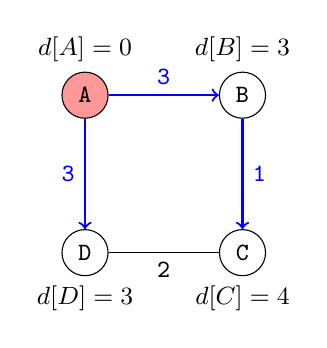
\begin{tikzpicture}
				\node[mynoder, label={above: \(d[A]=0\) }] at (0.0, 2.0) (a) {A};
				\node[mynode,  label={above: \(d[B]=3\) }] at (2.0, 2.0) (b) {B};
				\node[mynode,  label={below: \(d[C]=4\) }] at (2.0, 0.0) (c) {C};
				\node[mynode,  label={below: \(d[D]=3\) }] at (0.0, 0.0) (d) {D};
				\draw[edger] (a) edge node[above] {3} (b);
				\draw[edger] (b) edge node[right] {1} (c);
				\draw[edgen] (c) edge node[below] {2} (d);
				\draw[edger] (a) edge node[left] {3} (d);
			\end{tikzpicture}
\ifstandalone
		\end{subfigure}
	\end{figure}
\end{document}
\fi
